\documentclass{article}

% 中文支持设置
\usepackage{xeCJK}
\setCJKmainfont[BoldFont=SimHei,ItalicFont=KaiTi,AutoFakeBold=true,BoldItalicFont=SimHei]{SimSun} % 设置中文字体为宋体,粗体使用黑体
\setCJKsansfont[BoldFont=SimHei]{SimHei} % 设置中文无衬线字体为黑体
\setCJKmonofont[BoldFont=SimHei]{SimSun} % 设置中文等宽字体
\newCJKfontfamily\heiti[BoldFont=SimHei]{SimHei} % 设置黑体字体命令
\newCJKfontfamily\kaishu{KaiTi} % 设置楷体字体命令
\newCJKfontfamily\fangsong{FangSong} % 设置仿宋字体命令
\newCJKfontfamily\lishu{LiShu} % 设置隶书字体命令

% 页面设置
\usepackage[a4paper,top=2cm,bottom=2cm,left=3cm,right=3cm,marginparwidth=1.75cm]{geometry}

% 有用的包
\usepackage{amsmath}
\usepackage{amssymb}
\usepackage{graphicx}
\usepackage{longtable}
\usepackage{array}
\usepackage{booktabs}
\usepackage{xcolor}
\usepackage{colortbl}
\usepackage[colorlinks=true, allcolors=blue, unicode]{hyperref} % 添加 unicode 选项
\usepackage{listings}
\usepackage{float} % 添加 float 宏包
\usepackage{tocbibind} % 添加 tocbibind 宏包
\lstset{
      basicstyle=\ttfamily, % Use a monospaced font, similar to \verb
      breaklines=true,      % Allow automatic line breaking
      breakatwhitespace=false % Allow breaking anywhere, not just at spaces
}

% 中文标签设置
\renewcommand{\abstractname}{摘要}
\renewcommand{\contentsname}{目录}
\renewcommand{\listfigurename}{插图目录}
\renewcommand{\listtablename}{表格目录}
\renewcommand{\refname}{参考文献}
\renewcommand{\indexname}{索引}
\renewcommand{\figurename}{图}
\renewcommand{\tablename}{表}
\renewcommand{\appendixname}{附录}

\title{一篇示例文本}
\author{szw0407}
\usepackage{hyperref}
\begin{document}
\maketitle

\begin{abstract}
这是一个摘要。

在这里,您可以简要介绍您的文档内容、目的和主要结论。摘要通常是读者了解文档主题的第一步,因此请确保它简洁明了。
摘要通常包括研究的背景、方法、结果和结论。它应该足够简短,以便读者可以快速了解文档的核心内容。
\end{abstract}
\tableofcontents
\newpage
\section{引言}

您的引言在这里!只需开始编写您的文档并使用重新编译按钮查看更新的PDF预览。下面列出了常用命令和功能的示例,以帮助您入门。

一旦您熟悉了编辑器,您可以在Overleaf菜单中找到各种项目设置,该菜单可通过编辑器最左上角的按钮访问。要查看教程、用户指南和更多文档,请访问我们的\href{https://www.overleaf.com/learn}{帮助库},或前往我们的计划页面\href{https://www.overleaf.com/user/subscription/plans}{选择您的计划}。

\section{一些入门示例}

\subsection{如何创建章节和小节}

只需使用章节和小节命令,就像在这个示例文档中一样!使用Overleaf,所有格式和编号都会根据您选择的模板自动处理。如果您使用可视化编辑器,您也可以通过编辑器工具栏中的按钮创建新的章节和小节。

\subsection{如何包含图形}

首先,您必须使用文件树菜单中的上传链接从计算机上传图像文件。然后使用includegraphics命令将其包含在文档中。使用figure环境和caption命令为您的图形添加编号和标题。请参见本节中图\ref{fig:frog}的代码示例。

请注意,考虑到周围的文本以及可能附近的其他图形或表格,您的图形将自动放置在最合适的位置。您可以在这篇关于\href{https://www.overleaf.com/learn/how-to/Including_images_on_Overleaf}{在Overleaf上包含图像}的帮助文章中了解更多关于向文档添加图像的信息。

\begin{figure}
\centering
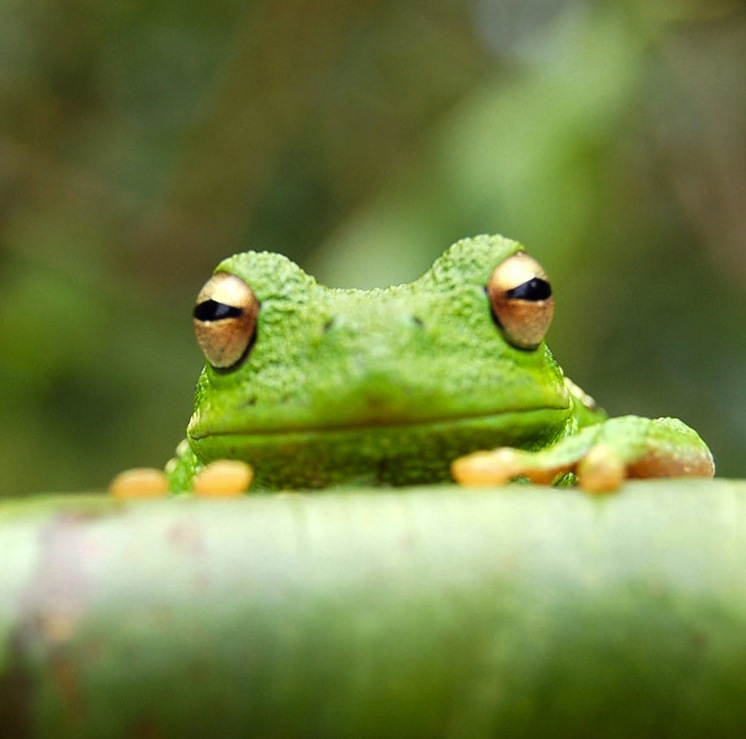
\includegraphics[width=0.25\linewidth]{frog.jpg}
\caption{\label{fig:frog}这只青蛙是通过文件树菜单上传的。}
\end{figure}

\subsection{如何添加表格}

使用table和tabular环境创建基本表格——例如表~\ref{tab:widgets}。更多信息,请参见这篇关于\href{https://www.overleaf.com/learn/latex/tables}{表格}的帮助文章。

\begin{table}
\centering
\begin{tabular}{l|r}
项目 & 数量 \\\hline
小部件 & 42 \\
小工具 & 13
\end{tabular}
\caption{\label{tab:widgets}示例表格。}
\end{table}

\subsection{如何添加注释和跟踪更改}

可以通过高亮显示一些文本并点击编辑器窗格右上角的"添加注释"来为您的项目添加注释。要查看现有注释,请点击上方工具栏中的审阅菜单。要回复注释,请点击注释右下角的回复按钮。当您暂时完成审阅时,可以通过点击工具栏上的名称来关闭审阅窗格。

跟踪更改功能在我们所有的\href{https://www.overleaf.com/user/subscription/plans}{高级计划}中都可用,可以使用审阅窗格顶部的选项来开启或关闭。跟踪更改允许您跟踪对文档所做的每一项更改,以及进行更改的人员。

\subsection{如何添加列表}

您可以制作自动编号的列表……

\begin{enumerate}
\item 像这样,
\item 也像这样。
\end{enumerate}
……或项目符号……
\begin{itemize}
\item 像这样,
\item 也像这样。
\end{itemize}

\subsection{如何编写数学公式}

\LaTeX{}在排版数学公式方面表现出色。设$X_1, X_2, \ldots, X_n$是一个独立同分布的随机变量序列,其中$\text{E}[X_i] = \mu$和$\text{Var}[X_i] = \sigma^2 < \infty$,设
\[S_n = \frac{X_1 + X_2 + \cdots + X_n}{n}
      = \frac{1}{n}\sum_{i}^{n} X_i\]
表示它们的均值。那么当$n$趋于无穷大时,随机变量$\sqrt{n}(S_n - \mu)$在分布上收敛到正态分布$\mathcal{N}(0, \sigma^2)$。

\subsubsection{矩阵示例}

考虑一个$3 \times 3$的矩阵$A$:
\[A = \begin{pmatrix}
1 & 2 & 3 \\
4 & 5 & 6 \\
7 & 8 & 9
\end{pmatrix}\]

矩阵的转置为:
\[A^T = \begin{bmatrix}
1 & 4 & 7 \\
2 & 5 & 8 \\
3 & 6 & 9
\end{bmatrix}\]

\subsubsection{公式推导示例}

推导二次方程的求根公式。对于方程$ax^2 + bx + c = 0$(其中$a \neq 0$),我们有:

\begin{align}
ax^2 + bx + c &= 0 \\
x^2 + \frac{b}{a}x + \frac{c}{a} &= 0 \\
x^2 + \frac{b}{a}x &= -\frac{c}{a} \\
x^2 + \frac{b}{a}x + \left(\frac{b}{2a}\right)^2 &= -\frac{c}{a} + \left(\frac{b}{2a}\right)^2 \\
\left(x + \frac{b}{2a}\right)^2 &= \frac{b^2 - 4ac}{4a^2} \\
x + \frac{b}{2a} &= \pm\frac{\sqrt{b^2 - 4ac}}{2a} \\
x &= \frac{-b \pm \sqrt{b^2 - 4ac}}{2a}
\end{align}

\subsubsection{逻辑运算示例}

设$P$和$Q$是两个命题,我们可以构造真值表来验证德摩根定律:$\neg(P \land Q) \equiv (\neg P) \lor (\neg Q)$

\begin{table}[h]
\centering
\begin{tabular}{|c|c|c|c|c|c|c|}
\hline
$P$ & $Q$ & $P \land Q$ & $\neg(P \land Q)$ & $\neg P$ & $\neg Q$ & $(\neg P) \lor (\neg Q)$ \\
\hline
T & T & T & F & F & F & F \\
T & F & F & T & F & T & T \\
F & T & F & T & T & F & T \\
F & F & F & T & T & T & T \\
\hline
\end{tabular}
\caption{德摩根定律的真值表验证}
\end{table}

从表中可以看出,$\neg(P \land Q)$和$(\neg P) \lor (\neg Q)$的真值完全相同,因此德摩根定律成立。

\subsubsection{命题逻辑推理示例}

考虑以下逻辑推理过程:

\textbf{前提:}
\begin{enumerate}
\item 如果下雨,那么地面湿润:$R \rightarrow W$
\item 如果地面湿润,那么道路滑:$W \rightarrow S$
\item 现在正在下雨:$R$
\end{enumerate}

\textbf{推理过程:}
\begin{align}
&\text{前提1:} R \rightarrow W \\
&\text{前提2:} W \rightarrow S \\
&\text{前提3:} R \\
&\text{步骤1:由前提1和前提3,应用分离规则:} W \\
&\text{步骤2:由前提2和步骤1结果,应用分离规则:} S \\
&\text{步骤3:由前提1和前提2,应用假言三段论:} R \rightarrow S
\end{align}

\textbf{结论:}道路滑($S$),且如果下雨则道路滑($R \rightarrow S$)。

\subsubsection{计算机算法复杂度分析}

考虑冒泡排序算法的时间复杂度分析:

\textbf{算法描述:}对于长度为$n$的数组,冒泡排序需要进行$n-1$轮比较,第$i$轮需要进行$n-i$次比较。

\textbf{复杂度推导:}
\begin{align}
T(n) &= \sum_{i=1}^{n-1} (n-i) \\
&= \sum_{j=1}^{n-1} j \quad \text{(令$j = n-i$)} \\
&= \frac{(n-1)n}{2} \\
&= \frac{n^2 - n}{2} \\
&= \frac{1}{2}n^2 - \frac{1}{2}n
\end{align}

因此,冒泡排序的时间复杂度为$O(n^2)$。

\textbf{空间复杂度:}由于只需要常数个额外变量进行交换操作,空间复杂度为$O(1)$。

\textbf{最佳情况分析:}当数组已经有序时,可以通过添加标志位优化,使最佳情况的时间复杂度降至$O(n)$。


\subsection{如何更改页边距和纸张大小}

通常您使用的模板会为该用例正确设置页边距和纸张大小。例如,如果您使用期刊出版商提供的期刊文章模板,该模板将根据他们的要求进行格式化。在这些情况下,最好不要直接更改页边距。

但是,如果您使用的是更通用的模板(如这个模板),并且想要更改页边距,常见的方法是通过geometry包。您可以在此示例文件顶部的前言中找到加载的geometry包,如果您想了解更多关于如何调整设置的信息,请访问这篇关于\href{https://www.overleaf.com/learn/latex/page_size_and_margins}{页面大小和页边距}的帮助文章。

\subsection{如何更改文档语言和拼写检查设置}

Overleaf支持许多不同的语言,包括在一个文档中使用多种不同的语言。

要配置文档语言,只需编辑此示例项目顶部前言中提供给babel包的选项。要了解更多不同选项,请访问这篇关于\href{https://www.overleaf.com/learn/latex/International_language_support}{国际语言支持}的帮助文章。

要更改拼写检查语言,只需打开编辑器窗口左上角的Overleaf菜单,向下滚动到拼写检查设置,并相应调整。

\subsection{如何添加引用和参考文献列表}

您可以简单地上传一个包含BibTeX条目的\verb|.bib|文件,该文件可以使用JabRef等工具创建。然后您可以引用其中的条目,就像这样:\cite{greenwade93}。只需记住指定参考文献样式以及\verb|.bib|文件的文件名。您可以在\href{https://www.overleaf.com/help/97-how-to-include-a-bibliography-using-bibtex}{这里找到视频教程}来了解更多关于BibTeX的信息。

如果您有\href{https://www.overleaf.com/user/subscription/plans}{升级账户},您也可以通过文件树中的上传菜单直接将您的Mendeley或Zotero库导入为\verb|.bib|文件。

\subsection{祝您好运!}

我们希望您觉得Overleaf有用,并且请查看我们的\href{https://www.overleaf.com/learn}{帮助库}获取更多教程和用户指南!如果您有任何反馈,请使用Overleaf菜单底部的\textbf{联系我们}链接,或使用\url{https://www.overleaf.com/contact}的联系表单。

\section{致谢}

在此文档的撰写过程中,我要特别感谢GitHub Copilot提供的智能编程辅助。作为一个AI编程助手,GitHub Copilot在代码生成、语法提示和问题解决方面给予了巨大帮助,显著提高了文档编写和代码开发的效率。

感谢GitHub Copilot团队开发了如此优秀的AI工具,让编程工作变得更加高效和愉快。

\bibliographystyle{alpha}
\bibliography{sample}

\appendix
\section{附录}
本节包含一些附加信息和示例,供需要时参考。
\section{LaTeX特殊符号速查表}

本节提供常用的LaTeX特殊符号速查表,方便快速查找和使用。

\subsection{数学符号}

\subsubsection{希腊字母}
\begin{table}[H]
\centering
\begin{tabular}{|c|c|c|c|c|c|}
\hline
小写 & 代码 & 大写 & 代码 & 小写 & 代码 \\
\hline
$\alpha$ & \verb|\alpha| & $\mathrm{A}$ & \verb|A| & $\nu$ & \verb|\nu| \\
$\beta$ & \verb|\beta| & $\mathrm{B}$ & \verb|B| & $\xi$ & \verb|\xi| \\
$\gamma$ & \verb|\gamma| & $\Gamma$ & \verb|\Gamma| & $o$ & \verb|o| \\
$\delta$ & \verb|\delta| & $\Delta$ & \verb|\Delta| & $\pi$ & \verb|\pi| \\
$\epsilon$ & \verb|\epsilon| & $\mathrm{E}$ & \verb|E| & $\rho$ & \verb|\rho| \\
$\zeta$ & \verb|\zeta| & $\mathrm{Z}$ & \verb|Z| & $\sigma$ & \verb|\sigma| \\
$\eta$ & \verb|\eta| & $\mathrm{H}$ & \verb|H| & $\tau$ & \verb|\tau| \\
$\theta$ & \verb|\theta| & $\Theta$ & \verb|\Theta| & $\upsilon$ & \verb|\upsilon| \\
$\iota$ & \verb|\iota| & $\mathrm{I}$ & \verb|I| & $\phi$ & \verb|\phi| \\
$\kappa$ & \verb|\kappa| & $\mathrm{K}$ & \verb|K| & $\chi$ & \verb|\chi| \\
$\lambda$ & \verb|\lambda| & $\Lambda$ & \verb|\Lambda| & $\psi$ & \verb|\psi| \\
$\mu$ & \verb|\mu| & $\mathrm{M}$ & \verb|M| & $\omega$ & \verb|\omega| \\
\hline
\end{tabular}
\caption{希腊字母符号表}
\end{table}

\subsubsection{数学运算符}
\begin{center}
\begin{tabular}{ccc|ccc}
\hline
\textbf{符号} & \textbf{代码} & \textbf{说明} & \textbf{符号} & \textbf{代码} & \textbf{说明} \\
\hline
$+$ & \verb|+| & 加法 & $\times$ & \verb|\times| & 乘法 \\
$-$ & \verb|-| & 减法 & $\cdot$ & \verb|\cdot| & 点乘 \\
$=$ & \verb|=| & 等于 & $\neq$ & \verb|\neq| & 不等于 \\
$<$ & \verb|<| & 小于 & $>$ & \verb|>| & 大于 \\
$\leq$ & \verb|\leq| & 小于等于 & $\geq$ & \verb|\geq| & 大于等于 \\
$\ll$ & \verb|\ll| & 远小于 & $\gg$ & \verb|\gg| & 远大于 \\
\hline
\end{tabular}
\end{center}

\subsubsection{集合与逻辑符号}
% 对于 longtable,它默认会尽可能保持在当前位置,如果需要更强的固定,可能需要其他方法或重构为 standard table
\begin{longtable}{|p{1.5cm}|p{2cm}|p{1.5cm}|p{2cm}|p{1.5cm}|p{2cm}|}
\hline
\multicolumn{6}{|c|}{\textbf{集合与逻辑符号对照表}} \\
\hline
\textbf{符号} & \textbf{代码} & \textbf{符号} & \textbf{代码} & \textbf{符号} & \textbf{代码} \\
\hline
\endfirsthead
\hline
\textbf{符号} & \textbf{代码} & \textbf{符号} & \textbf{代码} & \textbf{符号} & \textbf{代码} \\
\hline
\endhead
$\in$ & \verb|\in| & $\notin$ & \verb|\notin| & $\ni$ & \verb|\ni| \\
$\cap$ & \verb|\cap| & $\cup$ & \verb|\cup| & $\setminus$ & \verb|\setminus| \\
$\emptyset$ & \verb|\emptyset| & $\varnothing$ & \verb|\varnothing| & $\infty$ & \verb|\infty| \\
$\land$ & \verb|\land| & $\lor$ & \verb|\lor| & $\neg$ & \verb|\neg| \\
$\wedge$ & \verb|\wedge| & $\vee$ & \verb|\vee| & $\exists$ & \verb|\exists| \\
$\forall$ & \verb|\forall| & $\implies$ & \verb|\implies| & $\iff$ & \verb|\iff| \\
\hline
\end{longtable}

\subsubsection{积分与微分符号}
\begin{table}[H]
\centering
\begin{tabular}{>{\centering\arraybackslash}p{2cm}>{\centering\arraybackslash}p{3cm}>{\centering\arraybackslash}p{2cm}>{\centering\arraybackslash}p{3cm}}
\toprule
\textbf{符号} & \textbf{代码} & \textbf{符号} & \textbf{代码} \\
\midrule
$\int$ & \verb|\int| & $\iint$ & \verb|\iint| \\
$\iiint$ & \verb|\iiint| & $\oint$ & \verb|\oint| \\
$\sum$ & \verb|\sum| & $\prod$ & \verb|\prod| \\
$\coprod$ & \verb|\coprod| & $\bigcup$ & \verb|\bigcup| \\
$\bigcap$ & \verb|\bigcap| & $\bigoplus$ & \verb|\bigoplus| \\
$\partial$ & \verb|\partial| & $\nabla$ & \verb|\nabla| \\
\bottomrule
\end{tabular}
\caption{积分与微分符号}
\end{table}

\subsubsection{箭头符号}
\renewcommand{\arraystretch}{1.5}
\begin{table}[H]
\centering
\begin{tabular}{@{}lll@{}}
\toprule
\multicolumn{3}{c}{\textbf{箭头符号速查}} \\
\midrule
\textbf{水平箭头} & \textbf{垂直箭头} & \textbf{斜向箭头} \\
\midrule
$\rightarrow$ \verb|\rightarrow| & $\uparrow$ \verb|\uparrow| & $\nearrow$ \verb|\nearrow| \\
$\leftarrow$ \verb|\leftarrow| & $\downarrow$ \verb|\downarrow| & $\searrow$ \verb|\searrow| \\
$\leftrightarrow$ \verb|\leftrightarrow| & $\updownarrow$ \verb|\updownarrow| & $\nwarrow$ \verb|\nwarrow| \\
$\Rightarrow$ \verb|\Rightarrow| & $\Uparrow$ \verb|\Uparrow| & $\swarrow$ \verb|\swarrow| \\
$\Leftarrow$ \verb|\Leftarrow| & $\Downarrow$ \verb|\Downarrow| & \\
$\Leftrightarrow$ \verb|\Leftrightarrow| & $\Updownarrow$ \verb|\Updownarrow| & \\
\bottomrule
\end{tabular}
\caption{箭头符号分类表}
\end{table}
\renewcommand{\arraystretch}{1}

\subsection{文本符号}

\subsubsection{标点符号}
\begin{table}[H]
\centering
\begin{tabular}{|>{\columncolor{gray!20}}c|c|p{4cm}|p{4cm}|}
\hline
\rowcolor{gray!40}
\textbf{符号} & \textbf{代码} & \textbf{说明} & \textbf{示例} \\
\hline
"" & \verb|``''| & 英文双引号 & ``Hello World'' \\
\rowcolor{gray!10}
'' & \verb|`'| & 英文单引号 & `Hi there' \\
— & \verb|---| & 破折号 & Yes---or no? \\
\rowcolor{gray!10}
– & \verb|--| & 连接号 & pp. 13--67 \\
… & \verb|\ldots| & 省略号 & and so on\ldots \\
\rowcolor{gray!10}
§ & \verb|\S| & 段落符号 & \S1.2 \\
† & \verb|\dag| & 剑号 & text\dag \\
\hline
\end{tabular}
\caption{标点符号对照表}
\end{table}

\subsubsection{特殊字符}
\begin{table}[H]
\small
\centering
\begin{tabular}{*{6}{c}}
\hline
\multicolumn{6}{c}{\textbf{LaTeX特殊字符}} \\
\hline
\& & \% & \$ & \# & \_ & \textbackslash \\
\verb|\&| & \verb|\%| & \verb|\$| & \verb|\#| & \verb|\_| & \verb|\textbackslash| \\
\hline
\{ & \} & \^{} & \~{} & © & ® \\
\verb|\{| & \verb|\}| & \verb|\^{}| & \verb|\~{}| & \verb|\copyright| & \verb|\textregistered| \\
\hline
\end{tabular}
\caption{特殊字符速查}
\end{table}

\subsection{数学字体}

\subsubsection{字体样式对比}
\begin{table}[H]
\centering
\begin{tabular}{>{\bfseries}l|c|>{\ttfamily}l}
\hline
\textbf{字体类型} & \textbf{示例效果} & \textbf{LaTeX代码} \\
\hline
正体 & $\mathrm{ABC}$ & \verb|\mathrm{ABC}| \\
斜体 & $\mathit{ABC}$ & \verb|\mathit{ABC}| \\
粗体 & $\mathbf{ABC}$ & \verb|\mathbf{ABC}| \\
无衬线 & $\mathsf{ABC}$ & \verb|\mathsf{ABC}| \\
等宽 & $\mathtt{ABC}$ & \verb|\mathtt{ABC}| \\
花体 & $\mathcal{ABC}$ & \verb|\mathcal{ABC}| \\
空心 & $\mathbb{ABC}$ & \verb|\mathbb{ABC}| \\
哥特体 & $\mathfrak{ABC}$ & \verb|\mathfrak{ABC}| \\
\hline
\end{tabular}
\caption{数学字体样式对比}
\end{table}

\subsection{重音符号}

\subsubsection{数学重音符号}
\begin{center}
\footnotesize
\begin{tabular}{ccc|ccc|ccc}
\hline
\multicolumn{9}{c}{\normalsize\textbf{重音符号全览}} \\
\hline
\textbf{符号} & \textbf{代码} & \textbf{说明} & \textbf{符号} & \textbf{代码} & \textbf{说明} & \textbf{符号} & \textbf{代码} & \textbf{说明} \\
\hline
$\hat{a}$ & \verb|\hat{a}| & 帽子 & $\check{a}$ & \verb|\check{a}| & 检查 & $\tilde{a}$ & \verb|\tilde{a}| & 波浪 \\
$\acute{a}$ & \verb|\acute{a}| & 尖音 & $\grave{a}$ & \verb|\grave{a}| & 重音 & $\dot{a}$ & \verb|\dot{a}| & 单点 \\
$\ddot{a}$ & \verb|\ddot{a}| & 双点 & $\breve{a}$ & \verb|\breve{a}| & 短音 & $\bar{a}$ & \verb|\bar{a}| & 横线 \\
$\vec{a}$ & \verb|\vec{a}| & 向量 & & & & & & \\
\hline
\end{tabular}
\end{center}

\subsection{大型符号与括号}

\subsubsection{自适应括号示例}
\begin{table}[H]
\centering
\renewcommand{\arraystretch}{2.0}
\begin{tabular}{>{\centering}p{2cm}>{\centering}p{2cm}>{\centering\arraybackslash}p{8cm}}
\hline
\textbf{括号类型} & \textbf{自适应效果} & \textbf{代码} \\
\hline
圆括号 & $\left(\frac{a}{b}\right)$ & \lstinline|\left(\frac{a}{b}\right)| \\
\hline
方括号 & $\left[\frac{x^2}{y^2}\right]$ & \lstinline|\left[\frac{x^2}{y^2}\right]| \\
\hline
花括号 & $\left\{\frac{a}{b}\right\}$ & \lstinline|\left\{\frac{a}{b}\right\}| \\
\hline
角括号 & $\left\langle\frac{a}{b}\right\rangle$ & \lstinline|\left\langle\frac{a}{b}\right\rangle| \\
\hline
\end{tabular}
\caption{自适应括号效果对比}
\end{table}

\subsection{单位与常数}

\subsubsection{物理单位速查}
\begin{table}[H]
\centering
\renewcommand{\arraystretch}{1.3}
\begin{tabular}{||c|c||c|c||c|c||}
\hline\hline
\multicolumn{6}{||c||}{\textbf{国际单位制(SI)基本单位}} \\
\hline\hline
\textbf{物理量} & \textbf{单位符号} & \textbf{物理量} & \textbf{单位符号} & \textbf{物理量} & \textbf{单位符号} \\
\hline
长度 & $\text{m}$ & 质量 & $\text{kg}$ & 时间 & $\text{s}$ \\
\hline
电流 & $\text{A}$ & 温度 & $\text{K}$ & 物质量 & $\text{mol}$ \\
\hline
发光强度 & $\text{cd}$ & 频率 & $\text{Hz}$ & 力 & $\text{N}$ \\
\hline
能量 & $\text{J}$ & 功率 & $\text{W}$ & 压强 & $\text{Pa}$ \\
\hline\hline
\end{tabular}
\caption{物理单位对照表}
\end{table}

\subsubsection{数学常数汇总}
\begin{center}
\large
\begin{tabular}{@{}ccc@{}}
\toprule
\textbf{常数名称} & \textbf{符号} & \textbf{代码} \\
\midrule
圆周率 & $\pi \approx 3.14159$ & \verb|\pi| \\
自然对数底 & $e \approx 2.71828$ & \verb|e| \\
虚数单位 & $i^2 = -1$ & \verb|i| \\
无穷大 & $\infty$ & \verb|\infty| \\
空集 & $\emptyset$ & \verb|\emptyset| \\
偏微分算子 & $\partial$ & \verb|\partial| \\
梯度算子 & $\nabla$ & \verb|\nabla| \\
\bottomrule
\end{tabular}
\end{center}

\subsection{快速参考卡片}

\begin{table}[H]
\centering
\fbox{
\begin{minipage}{0.9\textwidth}
\textbf{LaTeX数学模式快速提示:}
\begin{itemize}
\item 行内公式:\texttt{\$...\$} 或 \texttt{\textbackslash(...\textbackslash)}
\item 行间公式:\texttt{\textbackslash[...\textbackslash]} 或 \texttt{\$\$...\$\$}
\item 编号公式:\texttt{\textbackslash begin\{equation\}...\textbackslash end\{equation\}}
\item 多行公式:\texttt{\textbackslash begin\{align\}...\textbackslash end\{align\}}
\item 矩阵:\texttt{\textbackslash begin\{pmatrix\}...\textbackslash end\{pmatrix\}}
\item 分式:\texttt{\textbackslash frac\{分子\}\{分母\}}
\item 上下标:\texttt{x\textasciicircum\{上标\}\textunderscore\{下标\}}
\item 根号:\texttt{\textbackslash sqrt[n]\{x\}}
\end{itemize}
\end{minipage}
}
\caption{LaTeX数学模式快速参考}
\end{table}
\end{document}
